
\subsection{2 模型架构}\label{model-architecture}

Kimi K3 架构从三个互补维度扩展信息流动：序列长度、网络深度和模型宽度。在序列维度上，Hybrid Attention 在每个 block 中将三层 Kimi Delta Attention (KDA) {[}63{]} 与一层 Gated MLA 结合，为长上下文 token 混合提供高效机制，同时保留选择性的高容量注意力（§2.1）。在深度维度上，Attention Residuals (AttnRes) {[}57{]} 使每个模块能够从嵌入层、当前 block 以及之前 block 中有选择地检索表示，将信息访问范围扩展到传统的顺序残差累积之外（§2.2）。在宽度维度上，每个注意力层之后跟随一个 Stable LatentMoE 层进行稀疏通道混合，为每个 token 有效地激活 896 个路由专家中的 16 个（§2.3）。对于原生视觉，MoonViT-V2 编码图像和视频，轻量级投影器将得到的视觉特征映射到共享嵌入空间，然后再进行 backbone 处理（§2.4）。结合 Per-Head Muon（§2.5），这些组件提供了一个统一的架构，用于在 token、层和通道之间扩展信息流动。结合精炼的训练和数据配方，它们使整体扩展效率相比 Kimi K2 提升约 2.5 倍。图 2 提供了架构概览。

\subsection{2.1 Hybrid Attention}\label{hybrid-attention}

Kimi K3 采用线性注意力与全局注意力的逐层混合，将 KDA {[}63{]} 与 Gated MLA 结合。每个 block 包含 3 个 KDA 层后接 1 个 Gated MLA 层，混合比例为 3:1。此模式在整个 backbone 中重复。两个注意力机制分别描述如下。在 backbone 末尾额外放置一个 Gated MLA 层，确保最后一层始终执行全局注意力。

\subsection{2.1.1 Kimi Delta Attention}\label{kimi-delta-attention}

KDA 将 delta-rule 递推 {[}105, 138{]} 与逐通道遗忘门 {[}63{]} 结合。考虑隐藏状态序列 \(\pmb { x } _ { t } \in \mathbb { R } ^ { d }\)，其中 t 索引 token 位置，d 是模型隐藏维度。为清晰起见，我们先描述单个注意力头，其 query 和 key 向量为 \(\boldsymbol { q } _ { t } , \boldsymbol { k } _ { t } \in \mathbb { R } ^ { d _ { k } }\)，value 向量为 \(\pmb { v } _ { t } \in \mathbb { R } ^ { d _ { v } }\)，递推状态为 \(\mathbf { S } _ { t } \in \mathbb { R } ^ { d _ { k } \times d _ { v } }\)。KDA 在 delta-rule 更新之前应用逐通道衰减：

\[
\mathbf {S} _ {t} = \left(\mathbf {I} - \beta_ {t} \boldsymbol {k} _ {t} \boldsymbol {k} _ {t} ^ {\top}\right) \operatorname{Diag} (\boldsymbol {\alpha} _ {t}) \mathbf {S} _ {t - 1} + \beta_ {t} \boldsymbol {k} _ {t} \boldsymbol {v} _ {t} ^ {\top}, \quad \tilde {\boldsymbol {o}} _ {t} = \mathbf {S} _ {t} ^ {\top} \boldsymbol {q} _ {t}.\tag{1}
\]

其中 \(\pmb { \alpha } _ { t } \in ( 0 , 1 ) ^ { d _ { k } }\) 是逐通道单步保留因子，\(\beta _ { t } \in ( 0 , 1 )\) 控制 delta-rule 写入强度。遵循 Kimi Linear {[}63{]}，KDA 将每头参数量参数化为

\[
\begin{array}{r l} & {\pmb {q} _ {t} ^ {h}, \pmb {k} _ {t} ^ {h} = \mathrm{L} _ {2} \mathrm{Norm} \Big (\mathrm{Swish} \Big (\mathrm{ShortConv} \Big (\mathbf {W} _ {q / k} ^ {h} \pmb {x} _ {t} \Big) \Big) \Big) \in \mathbb {R} ^ {d _ {k}},} \\ & {\pmb {v} _ {t} ^ {h} = \mathrm{Swish} \big (\mathrm{ShortConv} \big (\mathbf {W} _ {v} ^ {h} \pmb {x} _ {t} \big) \big) \in \mathbb {R} ^ {d _ {v}},} \\ & {\beta_ {t} ^ {h} = \mathrm{Sigmoid} \big (\mathbf {W} _ {\beta} ^ {h} \pmb {x} _ {t} \big) \in (0, 1),} \\ & {\pmb {z} _ {t} ^ {h} = \mathbf {W} _ {\alpha} ^ {\uparrow} \mathbf {W} _ {\alpha} ^ {\downarrow} \pmb {x} _ {t} + \pmb {b} _ {\alpha} ^ {h} \in \mathbb {R} ^ {d _ {k}}.} \end{array}\tag{2}
\]

query、key 和 value 投影先应用 ShortConv 再应用 Swish {[}138{]}，query 和 key 还通过 \(\mathrm { L _ { 2 } N o r m \bar { \lbrack 1 4 1 \rbrack } }\) 进行归一化。低秩投影和每头偏置 \(b _ { \alpha } ^ { h } \in \mathbb { R } ^ { d _ { k } ^ { \bullet } }\) 为每个 key 通道生成细粒度衰减 logit \$ \{ \boldsymbol { z } \} \_ \{ t \} \^{} \{ h \}\$。从 \$ \{ \boldsymbol { z } \} \_ \{ t \} \^{} \{ h \}\$ 到 \(\alpha _ { t } ^ { h }\) 的下界映射将在下文 chunkwise 公式之后引入。

Chunkwise 并行形式 遵循 Kimi Linear {[}63{]}，KDA 在 chunk 之间递推，在每个 chunk 内部并行。对于 chunk 大小 \(C , \mathbf { X } _ { [ t ] }\) 堆叠第 t 个 chunk 中的 token 向量，其中 \(\mathbf { X } \in \{ \mathbf { Q } , \mathbf { K } , \mathbf { V } , \mathbf { O } , \mathbf { \tilde { U } } , \mathbf { W } \}\)。矩阵 \(\mathbf { S } _ { [ t ] } \in \mathbb { R } ^ { d _ { k } \times d _ { v } }\) 表示进入 chunk t 的递推状态。对于位置 \(1 \leq i \leq j \leq C\)，定义逐通道累积衰减

\[
\gamma_ {[ t ]} ^ {i \rightarrow j} := \prod_ {r = i} ^ {j} \alpha_ {[ t ]} ^ {r}, \quad \gamma_ {[ t ]} ^ {r} := \gamma_ {[ t ]} ^ {1 \rightarrow r}.\tag{3}
\]

与 Kimi Linear 一样，\(\mathbf { \Gamma } _ { [ t ] } ^ { 1  C } \in \mathbb { R } ^ { C \times d _ { k } }\) 逐行堆叠 \(\gamma _ { [ t ] } ^ { 1 } , \ldots , \gamma _ { [ t ] } ^ { C }\)。UT 变换产生 \(\mathbf { U } _ { [ t ] }\) 和 \(\mathbf { W } _ { [ t ] }\)，由此定义伪 value 项 \(\widetilde { \mathbf { V } } _ { [ t ] } : = \mathbf { U } _ { [ t ] } - \mathbf { W } _ { [ t ] } \mathbf { S } _ { [ t ] }\)。给定传入状态 \({ \bf S } _ { [ t ] }\)，chunk t 中的所有输出并行计算为

\[
\begin{array}{l} \mathbf {A} _ {[ t ]} = \mathrm{Tril} \Big [ (\mathbf {Q} _ {[ t ]} \odot \mathbf {\Gamma} _ {[ t ]} ^ {1 \to C}) (\mathbf {K} _ {[ t ]} / \mathbf {\Gamma} _ {[ t ]} ^ {1 \to C}) ^ {\top} \Big ], \\ \mathbf {O} _ {[ t ]} = \underbrace {(\mathbf {\Gamma} _ {[ t ]} ^ {1 \to C} \odot \mathbf {Q} _ {[ t ]}) \mathbf {S} _ {[ t ]}} _ {\text {跨 chunk}} + \underbrace {\mathbf {A} _ {[ t ]} \widetilde {\mathbf {V}} _ {[ t ]}} _ {\text {chunk 内}}. \end{array}\tag{4}
\]

对于矩阵 M，Tril(M) 将所有严格上三角项置零，保留下三角项（包括对角线）。此 mask 强制 chunk 内的因果交互，对角线被保留是因为每个输出读取当前 token 更新之后的状态。\(\mathbf { O } _ { [ t ] }\) 中的第一项携带来自前面 chunk 的信息，而第二项则负责当前 chunk 内的交互。我们请读者参考 Kimi Linear {[}63{]} 了解 UT 变换和 chunkwise 形式的完整推导。

下界衰减 式 4 将每个 chunk 中的 key 按累积衰减的倒数 \(1 / \Gamma _ { [ t ] } ^ { 1  C }\) 重新缩放。由于 \(\Gamma _ { [ t ] } ^ { 1  C }\) 是 (0, 1) 范围内保留因子的乘积，这个倒数可以无限增长并在有限精度下溢出 {[}140, 63{]}。Kimi Linear 通过对数空间中的相对衰减计算并将每个 chunk 划分为次要的 16-token tile 来控制此数值范围 {[}140, 63{]}。非对角线 tile 可以直接用 Tensor Core 上的密集矩阵乘法计算。相比之下，对角线 tile 仍然需要显式的位置对计算，这仍然是主要的 chunk 内瓶颈。

\pandocbounded{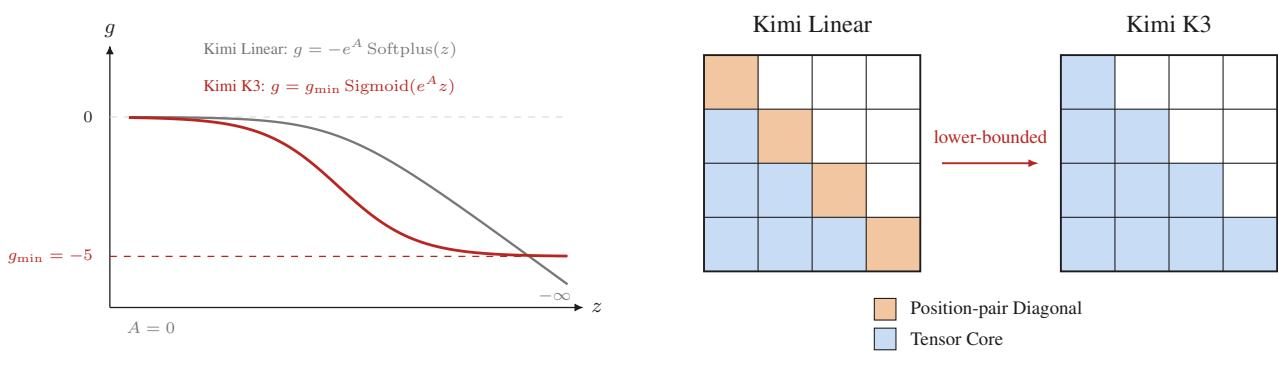
\includegraphics[keepaspectratio,alt={image}]{images/b25f80a09220511f967f568788cb62c2add55e59465c1b680077e6c6143a5bc0.jpg}}

\begin{enumerate}
\def\labelenumi{(\alph{enumi})}
\item
  对数衰减参数化。
\item
  对角线 tile 计算。
\end{enumerate}

图 3: 下界衰减及其对 chunkwise KDA 计算的影响。(a) Kimi Linear 使用无界负 Softplus 映射，而 Kimi K3 用缩放 sigmoid 限制对数衰减的下界；曲线显示 \(A = 0\) 和 \(g _ { \mathrm { m i n } } = - 5\)。(b) Kimi Linear 对每个对角线 tile 使用显式位置对计算，而 Kimi K3 中的有界范围允许所有因果 tile 使用密集 Tensor Core 矩阵乘法。

Kimi K3 通过改变从衰减 logit \(\boldsymbol { z } _ { t } ^ { h }\) 到每步对数衰减 \(\pmb { g } _ { t } ^ { h }\) 的映射来解决此瓶颈。遵循 GDN 和 Mamba-2，Kimi Linear 使用负 Softplus 映射 \(g _ { t } ^ { h } = - e ^ { A _ { h } }\) Softplus(zht ) ∈ \(( - \infty , 0 ) ^ { d _ { k } }\) {[}138, 24, 63{]}。Kimi K3 改用缩放 sigmoid 将对数衰减从下方约束：

\[
\begin{array}{r l} & {\pmb {g} _ {t} ^ {h} = g _ {\mathrm{min}} \mathrm{Sigmoid} \big (e ^ {A _ {h}} \pmb {z} _ {t} ^ {h} \big) \in (g _ {\mathrm{min}}, 0) ^ {d _ {k}},} \\ & {\pmb {\alpha} _ {t} ^ {h} = \exp (\pmb {g} _ {t} ^ {h}) \in (e ^ {g _ {\mathrm{min}}}, 1) ^ {d _ {k}},} \end{array}\tag{5}
\]

其中 \(A _ { h }\) 是可学习的每头对数尺度，\(g _ { \mathrm { m i n } } = - 5\) 是固定的。我们初始化 \(A _ { h } = 0 .\)，每个偏置 \(b _ { \alpha } ^ { h }\) 按照 {[}63, 24, 138{]} 初始化。在 \(g _ { \mathrm { m i n } } = - 5\) 下，每个保留因子满足 \(\alpha _ { t , j } ^ { h } > e ^ { - 5 } \approx 6 . 7 \times 1 0 ^ { - 3 }\)，16-token tile 上的累积对数衰减落在 \(( - 8 0 , 0 )\) 范围内。对应的倒数重缩放因子因此小于 \(e ^ { 8 0 }\)，保持在 BF16 动态范围内。这个有限范围使得对角线和非对角线 tile 都能使用密集 Tensor Core 矩阵乘法，消除了位置对对角线路径。此参数化与先前工作中的下界递推门 {[}97, 27, 91{]} 密切相关。图 3 说明了衰减参数化的变化及其计算后果。

全秩门控 最后，Kimi K3 将 KDA 的输出门从 Kimi Linear {[}63{]} 使用的低秩参数化改为输入依赖的全秩投影。在对递推输出应用逐头 RMSNorm {[}146{]} 之后，KDA 应用数据依赖的输出门控 {[}99{]}：

\[
\boldsymbol {y} _ {t} = \mathbf {W} _ {o} [ \mathrm{Sigmoid} (\mathbf {W} _ {g} \boldsymbol {x} _ {t}) \odot \mathrm{RMSNorm} (\tilde {\boldsymbol {o}} _ {t}) ].\tag{6}
\]

\subsection{2.1.2 Gated MLA}\label{gated-mla}

Multi-head Latent Attention (MLA)，由 DeepSeek-V2 {[}28{]} 引入，将每个 token 的 key--value 表示压缩到低维 latent 向量 \(\pmb { c } _ { t } = \mathbf { W } _ { c } \pmb { x } _ { t }\)。MLA 不缓存完整的每头 key 和 value，而是缓存 \(c _ { t }\)，并在注意力计算过程中通过学习的升维投影重建内容 key 和 value。这种分解减少了 KV-cache 占用，同时保留了全局 token-to-token 注意力。MLA 随后被 Kimi K2 和 Kimi K2.5 {[}58, 59{]} 采用，Kimi K3 在周期性全局注意力层中保留它。

与 Kimi K2 和 Kimi K2.5 不同，Kimi K3 遵循 Kimi Linear {[}63{]} 的混合设计，对所有 MLA 层应用 No Position Encoding (NoPE)。因此，不对其 query 或 key 应用任何显式位置编码。中间的 KDA 层提供位置敏感和近因感知的序列混合，而 MLA 层提供无限制的全局内容交互。这种分离还避免了在扩展上下文长度时修改位置编码参数，例如重新调整 RoPE 频率基或应用 YaRN {[}92{]}。

此外，Kimi K3 为 MLA 增加了一个输入依赖的、逐通道的全秩输出门。设 \({ \tilde { o } } _ { t }\) 表示位置 t 处未门控的 MLA 输出；门控输出为

\[
\boldsymbol {y} _ {t} = \mathbf {W} _ {o} [ \text {Sigmoid} (\mathbf {W} _ {g} \boldsymbol {x} _ {t}) \odot \tilde {\boldsymbol {o}} _ {t} ]  .\tag{7}
\]

门控投影 \(\mathbf { W } _ { g }\) 是全秩的，与 Kimi K3 中 KDA 使用的新参数化一致。此门控允许每个 token 调制从全局注意力读取的通道 {[}99{]}。

为纠正 flash attention 中出现的偏置舍入误差，我们采用 {[}98{]} 的方法，在训练期间将注意力输出保持在 FP32。此选择使输出 tile 的片上占用翻倍；因此我们重新设计了训练 kernel，将其与 KV staging buffer 而非 query tile 重叠，释放共享内存以支持更深的 KV 流水线和更高的训练吞吐量。

\subsection{2.2 Attention Residuals}\label{attention-residuals}

标准残差连接 {[}43{]} 将所有先前信息压缩到深度上的单个状态 \(h _ { l }\) —— 这是一个类似 RNN 在时间上的瓶颈。对于序列建模，Transformer 用注意力取代了递推 {[}10, 125{]}，允许每个位置用数据依赖的权重有选择地访问所有先前位置。Attention Residuals (AttnRes) {[}57{]} 将相同的方法应用于深度：每一层有选择地从所有先前层检索表示，而不是均匀地累积它们。

全注意力残差 对于每一层 l，我们定义层特定的可学习伪 query \(\pmb q _ { l } = \pmb w _ { l } \in \mathbb { R } ^ { d }\) 以及 key 和 value

\[
\boldsymbol {k} _ {i} = \boldsymbol {v} _ {i} = \left\{ \begin{array}{l l} \boldsymbol {h} _ {1} & i = 0 \\ f _ {i} (\boldsymbol {h} _ {i}) & 1 \leq i \leq l - 1 \end{array} \right.\tag{8}
\]

其中 \(f _ { i } ( h _ { i } )\) 是第 i 层的输出，\(\pmb { h } _ { 1 }\) 是 token 嵌入。注意力权重遵循 softmax 核 ϕ(q, k) = exp \(\left( \pmb q ^ { \top } \right)\) RMSNorm(k) {[}55, 146{]}，其中 RMSNorm 防止输出幅值较大的层主导权重：

\[
\alpha_ {i \rightarrow l} = \frac {\phi (\boldsymbol {q} _ {l} , \boldsymbol {k} _ {i})}{\sum_ {j = 0} ^ {l - 1} \phi (\boldsymbol {q} _ {l} , \boldsymbol {k} _ {j})}, \quad \boldsymbol {h} _ {l} = \sum_ {i = 0} ^ {l - 1} \alpha_ {i \rightarrow l} \cdot \boldsymbol {v} _ {i}.\tag{9}
\]

由于网络深度适中 \(( L < 1 0 0 )\)，这种全量形式的 \(O ( L ^ { 2 } d )\) 算术开销是可以接受的；实际开销是保持所有层输出活跃的 \(O ( L d )\) 内存（以及流水线并行下的跨阶段通信）。

Block 注意力残差 为降低此开销，我们将 L 层划分为 N 个 block，每个 block 含 \(S = L / N\) 层。在 block n 内（层索引 \(B _ { n } )\)），层输出通过求和归约为单个表示，\(b _ { n } =\) \(\textstyle \sum _ { j \in B _ { n } } f _ { j } ( h _ { j } )\)，其中 \({ b } _ { n } ^ { i }\) 表示 block 中前 i 层的部分和；我们设 \(b _ { 0 } = h _ { 1 }\) 使得 token 嵌入始终作为源被包含。跨 block，仅对 N 个 block 级表示应用全注意力：对于 block n 中的第 i 层，value 矩阵为

\[
\mathbf {V} = \left\{ \begin{array}{l l} [ \boldsymbol {b} _ {0}, \boldsymbol {b} _ {1}, \ldots , \boldsymbol {b} _ {n - 1} ] ^ {\top} & \text { 若 } i = 1 (\text { block } n \text { 的第一层}) \\ [ \boldsymbol {b} _ {0}, \boldsymbol {b} _ {1}, \ldots , \boldsymbol {b} _ {n - 1}, \boldsymbol {b} _ {n} ^ {i - 1} ] ^ {\top} & \text { 若 } i \geq 2 (\text { 后续层}) \end{array} \right.\tag{10}
\]

key 和注意力权重遵循式 8 和式 9。最终输出层随后聚合所有 N 个 block 表示。在 Block AttnRes 下，内存和通信开销从 \(O ( L d )\) 降至 \(\bar { \boldsymbol { O } } ( N d )\)，同时这种 block 结构还限制了推理时的状态，使得并行的跨 block 结果能够通过在线 softmax {[}79{]} 更好地与顺序的 block 内部部分和合并，显著减少推理时间成本。

经验上，\(N \approx { 8 }\) 在不同模型规模下恢复了大部分收益 {[}57{]}；对于 Kimi K3，我们将其层划分为 8 个 block，每个 block 12 层，形成不完整的最后一个 block 以及计入嵌入层后总共 9 个 block。

\subsection{2.3 Stable LatentMoE}\label{stable-latentmoe}

增加专家池和活跃专家数量可以扩展专家特化的空间，但在传统 MoE 中，每个被选中的专家接收完整的 d 维 token 表示，因此通信和专家权重流量随路由多重度增长。LatentMoE {[}32{]} 通过将完整模型宽度与路由专家宽度分离，使这种扩展变得经济可行：共享专家保留全宽路径用于常见变换，而特化的路由专家在宽度为 ℓ 的紧凑 latent 空间中运行。这使得 Kimi K3 能够将通道混合扩展到 896 个路由专家，每个 token 激活 16 个，对应的稀疏度为 56。

这种极端稀疏度放大了原始设计的两种失效模式。首先，路由路径将 \(\mathbf { W } ^ { \downarrow }\)、一个门控多分支专家前馈网络和 \(\mathbf { W } ^ { \uparrow }\) 组合成近四个连续矩阵乘法的链。这种病态结构，加上 2.8 万亿参数规模，在路由分支中产生爆炸式的内部激活。其次，平衡近 \(1 0 ^ { 3 }\) 个专家的负载超出了现有无辅助损失偏置更新保持良好行为的范围。Stable LatentMoE 通过三个组件应对这两种失效模式：在升维投影前的 RMSNorm 和 Sigmoid Tanh Unit GLU (SiTU-GLU) 用于抑制激活爆炸，以及 Quantile Balancing (QB) 用于负载均衡。

{\def\LTcaptype{none} % do not increment counter
\begin{longtable}[]{@{}llll@{}}
\toprule\noalign{}
\endhead
\bottomrule\noalign{}
\endlastfoot
& 门分支 & 升维分支 & 曲线 \\
GLU {[}26{]} & σ(x) & x &
\multirow{3}{*}{\pandocbounded{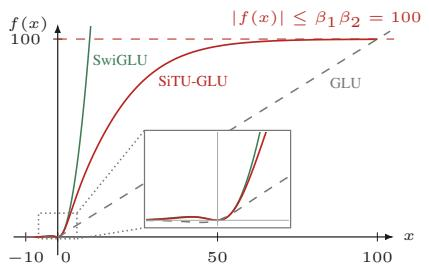
\includegraphics[keepaspectratio]{images/354bfbe64a6523e5071dd2734284728e26ea91d07069fdb6b7edfdc92b2deba4.jpg}}} \\
SwiGLU {[}107{]} & x·σ(x) & x \\
SiTU-GLU & β1 tanh(x/β1)·σ(x) & β2 tanh(x/β2) \\
\end{longtable}
}

图 4: GLU、SwiGLU 和 SiTU-GLU 的门分支和升维分支，及其标量响应，其中 \(\sigma\) 表示 sigmoid 函数。两个分支均接收标量输入 \(x ,\)，所有曲线共享定义域 \(x \in [ - 1 0 \widehat { , } 1 0 0 ]\)；插图为原点附近的放大视图。SiTU-GLU 以红色显示，\(\beta _ { 1 } = 4\) 和 \(\beta _ { 2 } = 2 5\)，在原点附近紧密跟随 SwiGLU，并且对于大的正输入趋近于界 \(| \bar { f } ( x ) | \overset { \cdot } { \leq } \beta _ { 1 } \beta _ { 2 } = 1 0 0\)，而 SwiGLU 保持无界。

如图 2 所示，该层遵循 DeepSeekMoE {[}23{]} 的共享与路由专家组织方式。对于 \(\pmb { x } \in \mathbb { R } ^ { d }\)，共享专家直接处理 x，而路由路径将其投影 \(\mathbf { \Gamma } _ { \mathrm { t o } } \mathbf { \check { z } } = \mathbf { W } ^ { \downarrow } \mathbf { \mathcal { x } } \in \mathbb { R } ^ { \ell }\)，将 z 分发给选中的专家，并通过 \(\mathbf { W } ^ { \uparrow }\) 将其加权聚合映射回 \(\mathbb { R } ^ { d }\)

\[
\begin{array}{l} \boldsymbol {u} = \sum_ {i \in \mathcal {T} _ {k} (\boldsymbol {x})} p _ {i} E _ {i} ^ {\text {routed}} (\mathbf {W} ^ {\downarrow} \boldsymbol {x}), \\ \boldsymbol {y} = \sum_ {j = 1} ^ {N _ {s}} E _ {j} ^ {\text {shared}} (\boldsymbol {x}) + \mathbf {W} ^ {\uparrow} \text {RMSNorm} (\boldsymbol {u}). \end{array}\tag{11}
\]

其中 \(\mathbf { \boldsymbol { u } } \in \mathbb { R } ^ { \ell }\) 是聚合后的路由表示，\(E _ { i } ^ { \mathrm { s h a r e d } } : \mathbb { R } ^ { d }  \mathbb { R } ^ { d }\) 和 Erouted : \(\mathbb { R } ^ { \ell } \to \mathbb { R } ^ { \ell }\) 分别是共享和路由专家前馈网络，\(p _ { i }\) 是下文 Quantile Balancing 规则定义的路由权重。Kimi K3 在每层固定全宽共享专家的数量为 \(N _ { s } = 2\)。

\subsection{2.3.1 Normalized LatentMoE}\label{normalized-latentmoe}

原始 LatentMoE 直接将 \(\mathbf { W } ^ { \uparrow }\) 应用于聚合后的路由表示 u，其尺度可能因所选专家及其路由权重而变化。如式 11 所示，Kimi K3 改为在专家聚合和升维投影之间插入 RMSNorm {[}146{]}。此归一化降低了路由分支对尺度变化的敏感性，使其在与全宽共享分支合并之前更加稳定。除了稳定训练外，额外的 RMSNorm 持续改善验证损失和下游基准。

\subsection{2.3.2 Sigmoid Tanh Unit GLU}\label{sigmoid-tanh-unit-glu}

Gated Linear Units (GLUs) 用 sigmoid 激活的门调制线性 value 分支，计算 \(\mathrm { S i g m o i d } ( \mathbf { W } _ { g } \pmb { x } ) \odot\) \({ \mathbf W } _ { u } \mathbf x\) {[}26{]}。SwiGLU 将 sigmoid 门替换为 Swish \(( x ) = x { \bar { \mathrm { S i g m o i d } } } ( x )\)，在 Transformer 中取得了很强的经验性能 {[}107{]}。SwiGLU 随后成为大语言模型中广泛采用的 FFN 设计，但对其经验有效性的完整解释仍然未决。

然而，SwiGLU 中的两个乘法因子都是无界的，因此重合的大值坐标可能导致激活异常值并增加低精度算术中的溢出风险。原始 GLU 的 sigmoid 门避免了门的无界增长，但它不保留 Swish 的近似线性正区间。这促使设计一种激活函数，在控制大值增长的同时保留 SwiGLU 的特征局部和正侧响应。最近的其他工作也探索了这种权衡的替代参数化 {[}51{]}。

为满足这些要求，我们提出了 Sigmoid Tanh Unit GLU (SiTU-GLU)。SiTU-GLU 将平滑上限 \(\mathrm { s o f t c a p } ( x , \beta ) = \dot { \beta } \mathrm { t a n h } ( x / \beta )\) 应用于 Swish 门的线性因子，并独立应用于升维分支：

\[
\text {SiTU - GLU} (\boldsymbol {x}) = \left[ \beta_ {1} \tanh \left(\frac {\mathbf {W} _ {g} \boldsymbol {x}}{\beta_ {1}}\right) \odot \text {Sigmoid} (\mathbf {W} _ {g} \boldsymbol {x}) \right] \odot \left[ \beta_ {2} \tanh \left(\frac {\mathbf {W} _ {u} \boldsymbol {x}}{\beta_ {2}}\right) \right],\tag{12}
\]

\pandocbounded{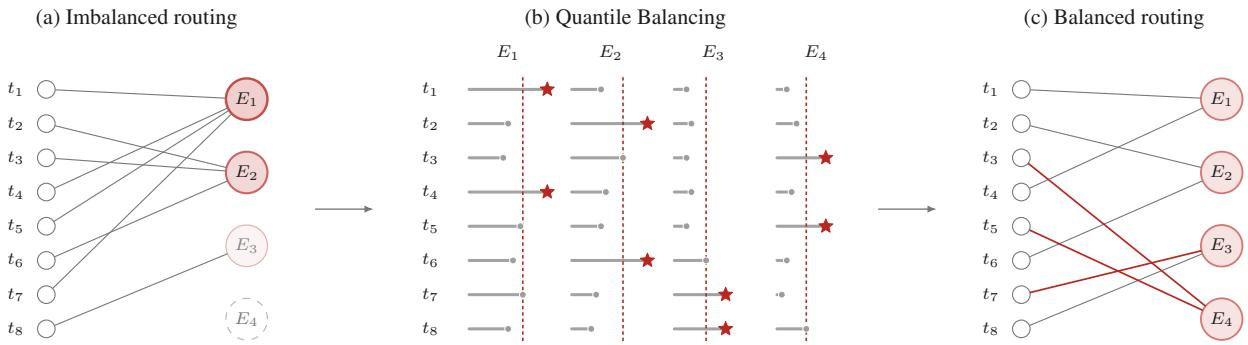
\includegraphics[keepaspectratio,alt={image}]{images/0a59b8921ae1851d33ec0e896c0bb7fdad30b2241c595d857542d84b609ddf67.jpg}}

图 5: Quantile Balancing 的示意，其中 \(m = 8\) 个 token，\(n = 4\) 个路由专家，每个 token 选择 \(k = 1\) 个专家。(a) 逐 token Top-k 路由（左侧为 token，右侧为专家）产生负载 \(( 4 , 3 , 1 , 0 )\)；较深的圆圈表示过热专家，而褪色和虚线圈分别表示未充分利用和消亡的专家。(b) 每个灰色条是当前偏置分数的 margin，\(s _ { i , j } + b _ { j } ^ { ( t ) } - \alpha _ { i } ^ { ( t ) }\)，因此逐行最大值再现了 (a) 中的路由。每列中的红色虚线是偏置调整 \(b _ { i } ^ { ( t ) } - \widehat { b } _ { i } ^ { ( t + 1 ) }\)，放置在 \(( q { + } 1 )\) 大的 margin 处，使得恰好 \(q = 2\) 个 margin 超过它。标记 ⋆ 表示减去列调整后的逐行 Top-k 选择，即 (c) 中的路由。(c) 保留的选择产生均衡负载 (2, 2, 2, 2)；红色边表示被 QB 改变的分派。

对于 Kimi K3，我们将 soft-cap 超参数设置为门分支 \(\beta _ { 1 } = 4\) 和升维分支 \(\beta _ { 2 } = 2 5\)。缩放 tanh 在原点附近近似线性，在大幅值时是有界的，使 SiTU-GLU 能够保留 SwiGLU 的局部响应，同时控制乘积中的两个因子。图 4 比较了 GLU、SwiGLU 和 SiTU-GLU 在公共切片上的分支定义和标量响应。

§ B 给出了局部展开、极限情况、形式化输出界以及与硬截断的比较。

\subsection{2.3.3 Quantile Balancing}\label{quantile-balancing}

与基于辅助损失的路由 {[}33{]} 不同，Kimi K3 采用无辅助损失路由 {[}30{]}。负载均衡通过向用于 Top-k 选择的路由分数添加专家特定偏置 \(b _ { j }\) 实现。对于 token xi，路由计算 \(s _ { i } = \mathrm { S i g m o i d } ( \mathbf { W } _ { r } \mathbf { x } _ { i } )\) 并应用

\[
\mathcal {T} _ {i} = \operatorname{argtop} _ {k} (\boldsymbol {s} _ {i} + \boldsymbol {b}), \qquad p _ {i, j} = \frac {\boldsymbol {s} _ {i , j}}{\sum_ {r \in \mathcal {T} _ {i}} s _ {i , r}}, \quad j \in \mathcal {T} _ {i}.\tag{13}
\]

因为 b 在 \(p _ { i , j } .\) 中被省略，它调节分派而不改变混合权重或路由器的梯度优化。原始方法用固定步长规则更新 b：\(b _ { i } ^ { ( t + 1 ) } = b _ { i } ^ { ( t ) } + \gamma \mathrm { s i g n } ( \bar { \ell } - \ell _ { i } ^ { ( t ) } )\) {[}30{]}，其中 γ 在缓慢适应和负载振荡之间权衡。当 LatentMoE 将每层路由专家池增加到 896 时，保持均衡负载变得更具挑战性。不均衡的路由会减慢专家并行训练，并可能使某些专家训练不足 {[}47{]}。

为了解决此限制，我们引入 Quantile Balancing (QB)，它从匹配目标负载的路由分数量化点设置每个专家偏置 {[}111{]}。考虑一个训练批次包含 m 个 token，路由到 n 个专家，使用 Top-k 选择，因此目标负载为每个专家 \(q : = m k / n\) 个 token。QB 通过单次前向传播推导下一个偏置。路由将 Top-k 选择替换为对有偏分数 \(s _ { i } + b ^ { ( t ) }\) 的 \(\mathrm { T o p } \mathrm { - } ( k { + } 1 )\)：前 k 个条目是实际采用的路由，而第 (k+1) 个条目是截止值 \(\alpha _ { i } ^ { ( t ) }\)，专家必须超过它才能进入 token i 的 Top-k。从 \(\mathrm { T o p } \mathrm { - } ( k { + } 1 )\) 路由取截止值避免了单独的 token 侧分位点。然后我们选择每个专家偏置，使得专家 \(j\) 达到其目标负载：在截止值固定的情况下，在候选偏置 \(\widehat { b } _ { j } ^ { ( t + 1 ) }\) 下路由到专家 \(j\) 的 token 计数为

\[
\sum_ {i = 1} ^ {m} \mathbf {1} \Big [ s _ {i, j} + \widehat {b} _ {j} ^ {(t + 1)} > \alpha_ {i} ^ {(t)} \Big ],
\]

该计数关于阈值 \(- \widehat { b } _ { j } ^ { ( t + 1 ) }\) 单调递减。假设无平局，将此计数设为 q 使得 \(- \widehat { b } _ { j } ^ { ( t + 1 ) }\) 成为第 (q+1) 大的 margin \(s _ { i , j } - \alpha _ { i } ^ { ( t ) }\)，从而恰好 q 个 margin 保持在阈值之上。由于 \(q / m = k / n\)，这是跨 token margin 的 \(( 1 - k / n )\) 分位数，给出 QB 更新

\[
\begin{array}{l} \widehat {b} _ {j} ^ {(t + 1)} \leftarrow - \text {quantile} _ {1 - k / n} \Big (\boldsymbol {s} _ {:, j} - \boldsymbol {\alpha} ^ {(t)} \Big), \\ \boldsymbol {b} ^ {(t + 1)} \leftarrow \widehat {\boldsymbol {b}} ^ {(t + 1)} - \text {mean} \Big (\widehat {\boldsymbol {b}} ^ {(t + 1)} \Big)   \mathbf {1}. \end{array}\tag{14}
\]

margin 从原始分数 \(s _ { i , j }\) 中减去有偏截止值 \(\alpha _ { i } ^ { ( t ) }\)，因此旧偏置仅通过截止值影响更新，第二行移除不影响 Top-k 选择的公共偏移。为保证因果性，更新仅在下一步生效 {[}30{]}，即批次从不使用从其自身推导的偏置进行路由。图 5 说明了 \(m = 8 , n = 4\) 和 \(k = 1\) 的情况，其中每个专家获得目标负载 \(q = 2 ,\)。最终偏置在推理时冻结。均衡分派的推导见 \(\ S \subset\)

直方图估计 在大规模下，式 14 中的分位数跨越整个全局批次，其 margin 数量达数百万并分布在多个 rank 和累积步骤中，因此在训练时收集它们进行精确分位数计算是不可行的。我们改为从每个专家的 margin 直方图中读取分位数：单次 all-reduce 汇总每 rank 的 bin 计数，分位数从汇总计数中恢复。由于计数是可加的，直方图表示汇聚后的全局批次，无论 token 如何分片，因此估计反映了全局批次分位数（精确到 bin 宽度），通信开销仅为每个专家几百个 bin。此直方图估计器是我们在实践中使用的方法；我们在 § D 中给出其详细描述及误差界。

\subsection{2.4 原生视觉}\label{native-vision}

Kimi K3 是原生多模态的：文本、图像和视频在单个上下文中由单一共享 backbone 处理，无需后置模态对齐阶段。此设计是 §1 中描述的长时间视野、循环中视觉行为（vision-in-the-loop）的架构基础。渲染输出及其产生代码存在于同一 token 流中，模型可以编写代码、检查结果的截图或视频帧，并迭代优化视觉产物——用户界面、图形、视频——无需跨模型交接。

MoonViT-V2 Kimi K2.5 的一个关键不同之处在于，我们使用下一 token 预测从头训练 Kimi K3 的视觉编码器 MoonViT-V2。先前的实践（包括 Kimi K2.5 本身）用对比预训练模型（如 SigLIP）初始化视觉编码器，前提是预训练的视觉知识能给模型带来先发优势。我们偏离此实践主要是为了训练稳定性。当预训练编码器附加到 LLM 时，联合优化变得不稳定：SigLIP 初始化的 MoonViT-3D 显示出持续更高的梯度范数，并伴随频繁的尖峰，而 MoonViT-V2 在整个训练过程中保持稳定（图 6）。使用下一 token 预测训练还允许编码器的表示直接由语言建模目标塑造，而不是由偏向全局语义而非细粒度文本和结构线索的对比损失来塑造。值得注意的是，我们发现 MoonViT-V2 在各种视觉评估上与 SigLIP 初始化的基线持平，表明在大规模多模态语言模型中对比预训练作为初始化是不必要的。

\begin{enumerate}
\def\labelenumi{(\alph{enumi})}
\item
  完整训练轨迹
\item
  放大视图（14k--16k）
\end{enumerate}

\pandocbounded{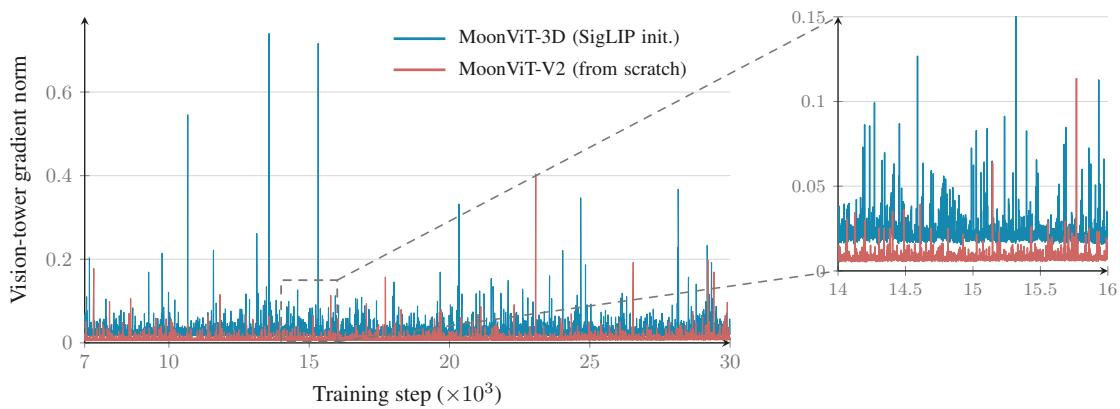
\includegraphics[keepaspectratio,alt={image}]{images/324bb9a298b4ef02fffcfe0b06951246aec549feb07deffd7c73da1b25884824.jpg}}

图 6: 预训练消融实验中的视觉塔梯度范数。与 SigLIP 初始化的 MoonViT-3D 相比，从头训练的 MoonViT-V2 保持更低的梯度范数和更少的尖峰，表明优化更加稳定。

架构 此训练方案建立在遵循 Kimi K2.5 {[}59, 61{]} 整体设计的视觉通路上：视觉输入首先由 MoonViT-V2 编码，然后通过轻量级 MLP 投影器映射到 LLM。MoonViT-V2 是一个 27 层的 vision transformer，参数约 0.4B，采用 RMSNorm 并从其线性和注意力投影中移除所有偏置项，这一设计进一步稳定了上述的从头优化。图像和视频以完全共享的参数处理，如 MoonViT-3D 中一样：注意力分解为帧内空间和帧间时间传递，时间池化进一步沿时间维度压缩 token。在投影之前，带有 2 2 下采样的 pixel-shuffle 操作将视觉 token 数量减少四倍，使高达 3584 3584 像素的输入在 1M-token 上下文中仍然可行。

\subsection{2.5 Per-Head Muon}\label{per-head-muon}

遵循 Kimi K2，Kimi K3 采用 Muon {[}53{]} 作为矩阵参数的优化器。对于注意力投影，我们将其进一步细化为 per-head 变体：不是将 Newton--Schulz 正交化应用于完整的 Q、K 和 V 投影矩阵，而是沿着 head 维度划分它们的动量矩阵，并分别对每个 head 的块进行正交化。其直觉是全矩阵正交化将所有 head 视为单一耦合块，因此梯度或动量尺度较大的 head 主导共享的更新方向，而尺度较小的 head 获得的归一化更新不足；per-head 正交化均衡了各 head 之间的更新尺度。在实践中，此设计产生了更均衡的跨 head 学习动态，并在更大规模上提高了训练稳定性。它还略微降低了优化器开销，因为在 tall per-head blocks 上的 Newton--Schulz 迭代比对完整投影矩阵计算更便宜。
